%
% latex-sample.tex
%
% This LaTeX source file provides a template for a typical research paper.
%

%
% Use the standard article template.
%
\documentclass{article}

% The geometry package allows for easy page formatting.
\usepackage{geometry}
\geometry{letterpaper}

% Load up special logo commands.
\usepackage{doc}

% make a reference to Hypertext 
\usepackage{hyperref}

% Package for formatting URLs.
\usepackage{url}

% Packages and definitions for graphics files.
\usepackage{graphicx}
\usepackage{epstopdf}
\DeclareGraphicsRule{.tif}{png}{.png}{`convert #1 'dirname #1'/'basename #1 .tif'.png}

%
% Set the title, author, and date.
%
\title{Caesar Hotel  \\ \small{DNSC 6211: Programming for Analytics}}
\author{
    Akash Bose \\
	Yatao Lu \\
	Xinyi Lu \\
	Zhencun Liu \\
}
\date{}

%
% The document proper.
%
\begin{document}

% Add the title section.
\maketitle

% Add an abstract.
\abstract{
The scope of this project is to develop an accurate forecast model for guest arrivals to Caesar's, Las Vegas, which shall then be used to optimize the front desk staffing model. We chose this project because it is an actual operational problem faced by Caesar's and many other hospitality services company. To execute this project, we purchased approximately 4 years of rewards member check-in data from Caesar's. Using Python and R-programming, we developed two forecast models, the moving average model and the casual model, to predict the number of check-ins on any given day. Model comparison shows us that there is not enough difference to be reasonably sure that one model is significantly better than the other. The purpose of this project is to forecast guest arrivals, and not to choose a model for further analysis and optimization. Further, statistical analysis is required to refine the model framwork and increase predictive power.
}

% Add various lists on new pages.
\pagebreak
\tableofcontents


% Start the paper on a new page.
\pagebreak

%
% Body text.
%
\section{Introduction}
\label{introduction}

Ensuring sufficient front desk staff is crucial to the customer experience, in addition, front desk staff at hotels in United States are usually unionized, which demands work schedule to be in place at least two weeks in advance. If the front desk is understaffed, guests will experience longer check-in time, which will impact their experience and impression at the hotel, leading to potential revenue loss for the hotel. On the other hand, if the front desk is overstaffed, hotels will usually suffer from higher cost. The staffing problem is one of the common examples of operations research domain and this project answers the forecasting part of the optimization problem.


\section{Background}

Caesar spent around 2 billion dollars annually on staffing and staffing-related expenses in 2012, which is the most significant factor leading to its net loss. Therefore we would like to simulate and forecast its front-desk staffing model to help reduce the costs. In order to do so, we will forecast its number of daily check-ins using appropriate statistical methods.Here are the key questions we will focus on:
How to define and analyze the independent variables with statistical significance? 
How to accurately forecast guest arrivals on a daily basis?
How accurate are our forecast models?


\section{Method}
Our methodology: 
\begin{itemize}
  \item  Pre-analysis of our data sets to see a high level distribution check-ins.
  \item Multivariate analysis of our data to test if there is a repeating independent variable, which may lead to multi-collinearity. 
  \item Multiple regression analysis using R
  \item Moving average model using Excel
  \item Compare forecast models to test the accuracy of our predictions using mean absolute percentage error (MAPE). Other metrics, such as sum of square errors (SSE), etc. can also be used.
\end{itemize} 

\section{Organization}

All our group members helped to find the right data set. Akash, Yatao and Xinyi did the programming part of project. Akash did the background analysis, all the histograms plots and the linear modeling in R; Yatao did the boxplot and Multi-variate analysis; Xinyi did the dotplot, time-series forecast models and R-shiny plots. For the write-up, Akash did the Abstract, Introduction, and proof-reading / editing; Yatao did the Methodology part. Akash helped the conclusion part. Xinyi finished all the remaining parts and finalized the report. Ashley initially wrote the abstract, introduction, workflow and conclusion but it needs to be rewritten. Akash finished the final video recording. 
 

\subsection{Workflow}

\begin{figure}[!htbp]
  \centering
    \includegraphics[height=7cm]{FlowChart}
  \caption{The project workflow}

\end{figure}


There are three main steps we executed. For pre-analysis exploration part, we explored the relationship of variables via histograms, boxplot and multivariate plot. Following this pre-analysis exploration, we utilized R to develop the multiple linear regression model. We also developed interative regression plot through R-shiny. This led us to the final forecast and visualization. In this part, we used dotplot to visualize coefficient strength of each independent variables. Finally, we utilized both Time-series model and Casual model to forecast the number of check-ins.



\subsection{Project structure}

Our main data source comes from the Caesar's inner database gathered from Analytical Department. The data includes a lot of categorical dummy variables like month, year and holidays. The number of customers coming to hotel is closely related to the free time they have and therefore these dummy variables are crucial to our analysis. The continuous variables include different customer types such as free and independent customers and Caesar's own Loyalty program customers. Different customers type will have different implication on the time they come to hotel and how much money they are willing to spend per night. At the same time, the multivariate regression gives us a very small p-value. Therefore we are reasonably sure that all these 50 variables have some statistical significance to our model.


\subsection{Figures and Tables}
For variables Day, Month, Year and Holidays, we plot histograms to show their relationship between number of Check-ins and each of the variables. Figure 1 to Figure 5 are histograms showing the number of Check-ins associated with Year, Month, Day and Holidays. 

\begin{figure}[!htbp]
  \centering
    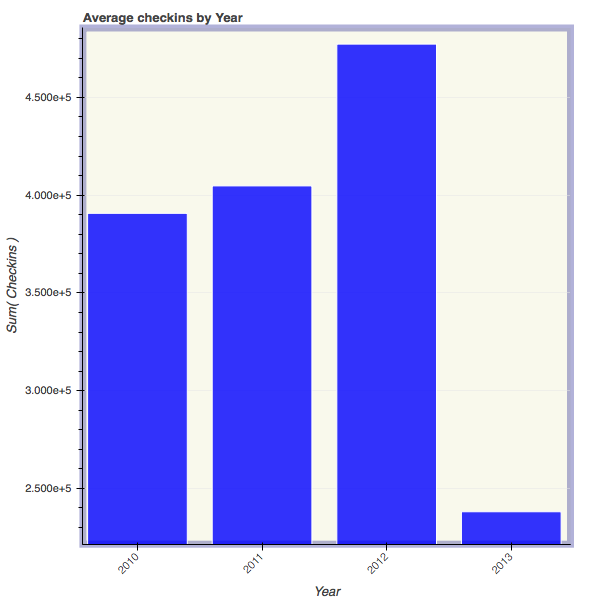
\includegraphics[height=5cm]{Hist_Yearly}
  \caption{Histogram on Yearly checkins}

\end{figure}

\begin{figure}[!htbp]
  \centering
    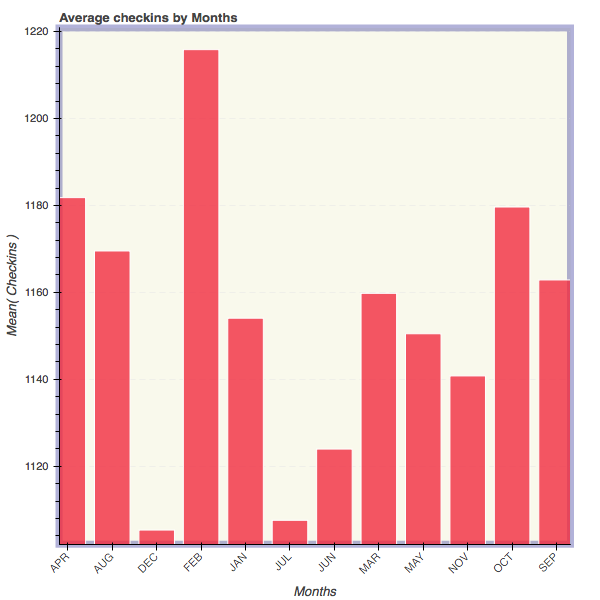
\includegraphics[height=5cm]{Hist_Monthly}
  \caption{Histogram on Monthly checkins}

\end{figure}

\begin{figure}[!htbp]
  \centering
    \includegraphics[height=5cm]{Hist_Daily}
  \caption{Histogram on Daily checkins}

\end{figure}

\begin{figure}[!htbp]
  \centering
    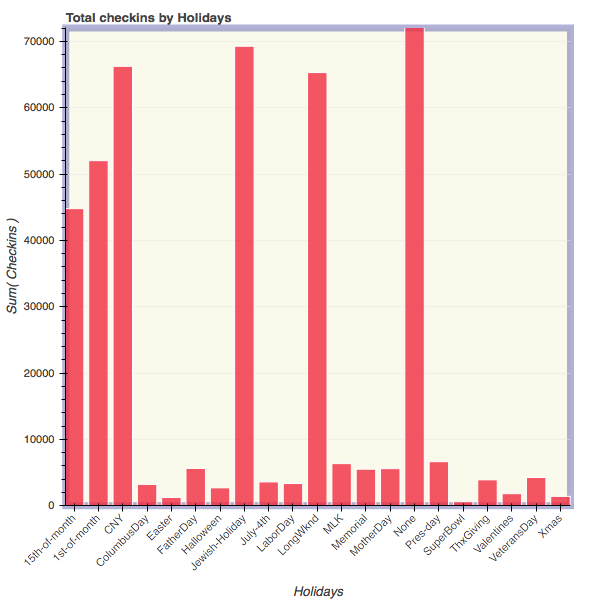
\includegraphics[height=5cm]{Hist_Holiday}
  \caption{Histogram on Holiday checkins}

\end{figure}
 
\begin{figure}[!htbp]
  \centering
    \includegraphics[height=3cm]{holiday}
  \caption{Boxplot on Month}

\end{figure}

\begin{figure}[!htbp]
  \centering
    \includegraphics[height=3cm]{month}
  \caption{Boxplot on Month continued}

\end{figure}

\begin{figure}[!htbp]
  \centering
    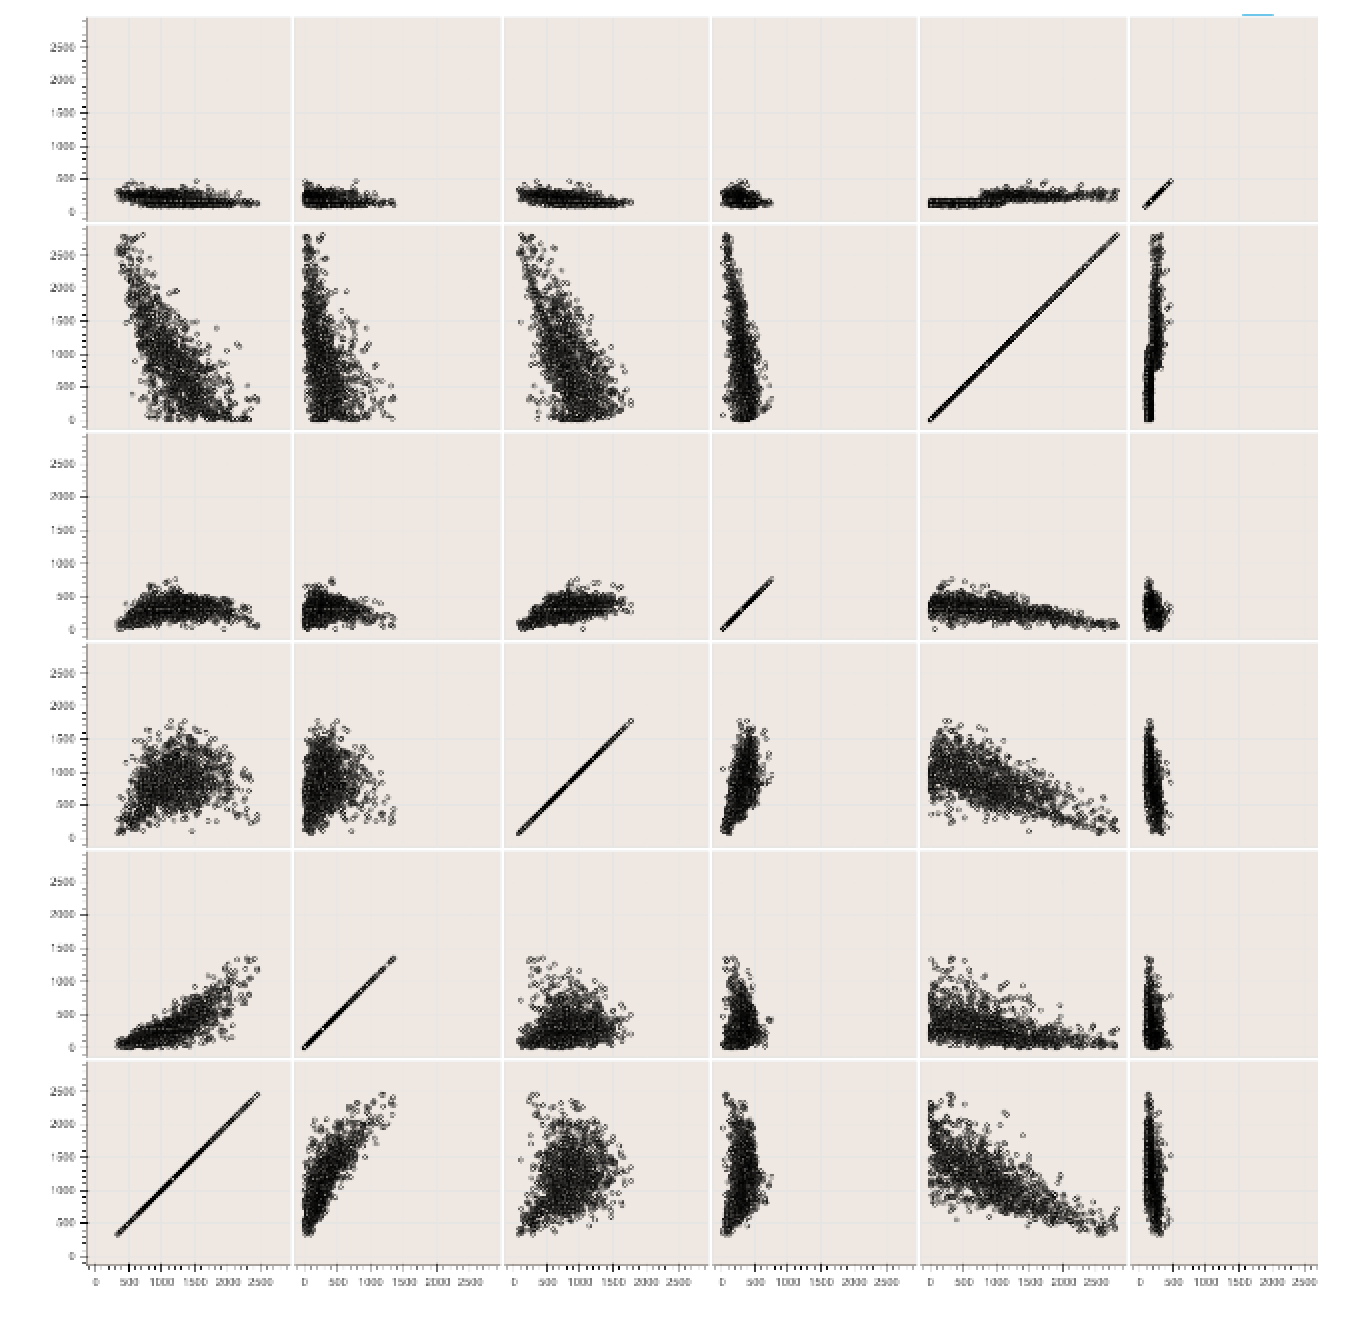
\includegraphics[height=8cm]{multi-v}
  \caption{Multivariate Analysis}

\end{figure}

\begin{figure}[!htbp]
  \centering
    \includegraphics[height=6cm]{R-shiny_plot}
  \caption{Sample Interactive R-shiny Regression Plot}
\end{figure}

\begin{figure}[!htbp]
  \centering
    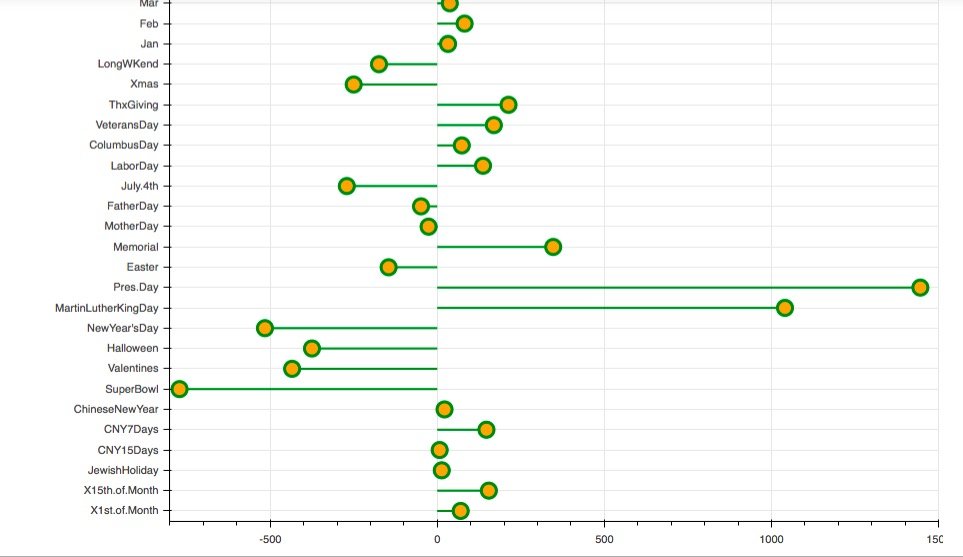
\includegraphics[height=6cm]{DotPlot}
  \caption{Sample Dotplot on Coefficient Strength}
\end{figure}

\begin{figure}[!htbp]
  \centering
    \includegraphics[height=6cm]{ActualAndMA}
  \caption{Time-Series Forecast}
\end{figure}

\begin{figure}[!htbp]
  \centering
    \includegraphics[height=6cm]{ActualAndReg}
  \caption{Causal Forecast}
\end{figure}

\begin{figure}[!htbp]
  \centering
    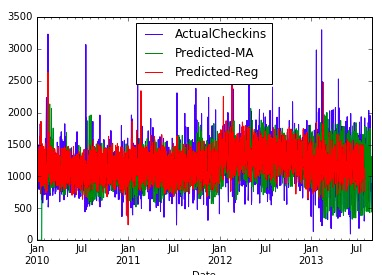
\includegraphics[height=6cm]{ForecastModels}
  \caption{Forecast Model}
\end{figure}

\begin{figure}[!htbp]
  \centering
    \includegraphics[height=6cm]{MAPE}
  \caption{Mean Absolute Error}
\end{figure}

The boxplots help us identify whether the data of the variables are equally distributed. For example in Figure 6, here we are comparing the number of check-ins in January vs. other months and looks like the distribution of check-ins is very similar, although January seems to have a lower average check-ins. Similarly, we find Sundays have a significantly higher check-ins than the other days. The purpose is to see the variance of check-ins on a given day and to see how it may influence the linear model coefficients. A small variance will invariably lead to a large coefficient and vice versa.
The Figure 9 is a demonstration of how we could plot the regression line associated with continuous variables.
Figure 10 show the plots of the coefficients of all the independent variables.
Figure 11 and 12 are the demonstration of our forecasts. The orange dots are our fore-casted number of customer check-ins and the blue dots are the actual number of check-ins.
Figure 13 shows our forecast models. We could find that Casual model(Red color) fits the actual data better. One possible improvement is that we could increase the confidence interval to fit more actual data. 
Figure 14 shows the Mean Absolute Errors for both of the forecasting models. Clearly causal model has a smaller error compared to the Time-series model.

\section{Discussion}

Our project focuses on a real industry case, which is how to help hotel better prepare their staffing model. We have over fifty independent variables so it is a difficult decision to figure out the key driver associated with the dependent variable, which is the number of daily check-ins. The biggest selling point is our utilization of multiple visualization tools, which help us to clearly see and identify the relationship between different variables and how strong they are correlated. For example, the histograms vividly show the number of check-ins associated with different year, month, day and even holidays. Thus from the graph we could know that Christmas has weigh more daily check-ins compared to the other holidays and we should place more from staff during this period. The second selling point is that we used both Time-series model and Casual relationship model to simulate and forecast the number of check-ins. It is interesting to plot the two forecast models and actual number together in one graph.

\subsection{Learnings}

We quite enjoyed the learning-by-doing process in order to show interactive and fun visualization to our peers. We have compared several visualization galleries, such as Bokeh and Lightening by Nate Silver. And finally we have chosen Bokeh as our main visualization tools because its gallery includes a lot of tools for statistical analysis. For example, after we finished all the regression, we used a dotplot(Figure 10) method to show the coefficients of all the independent variables. The direction of the dot and the line implies if the variable is positive or negative related the the number of check-ins. The length of the line implies how far the variable will affect a unit of the dependent variable. Th negative line of Valentines Day could imply that the people are willing to spend the day at home. Therefore the hotel should note spend too much resource on this holiday.

\subsection{Challenges}

We have not learned how to do Time-series forecast so we got a lot of help from Professor Kanungo. The video and resources he gave us are very useful for us in completing our project. In the programming session, we have difficulty in applying new visualization packages to give different plots. Fortunately we discussed and helped each other and successfully make our codes working. Mostly importantly, solving the front desk staffing problem relied heavily on being able to accurately forecast guest arrivals on a daily basis, and then break that down by staffing shifts. However there were many variables, outlier events and uncertainties that made forecasting difficult. Therefore, we completed both Time-series and regression forecasts and compared both of their results.


\section{Conclusion}

Ensuring optimal front desk staff is crucial to hotel and customer alike. We approached this problem by using statistical models to forecast daily guest check-ins by exploring daily check-ins from actual datas set from Caesar’s with the utilization of Python, R and Excel. We were then able to produce a causal forecast with 0.25 MAPE(Figure 14) with an adjusted R-square of 0.41; moving forward, this model can be improved by further statistical analysis. 

Our Jupyter notebook can be checked out there: \url{https://nbviewer.jupyter.org/github/bosea3000/Projects/blob/master/Caesars-Staffing-Problem/Checkin-Forecast.ipynb}

Our video can be checked out there: \url{https://youtu.be/OynwhL2hDWE}


\end{document}

